\section{Simulación}\label{sec:simulacion}
\begin{frame}{Parámetros del sistema}
    \begin{block}{Parámetros fijos}
        \begin{itemize}
            \item Dimensiones de la cancha - 100\ m x 70\ m\)
            \item Velocidad máxima de los jugadores azules - \(v_{azul}^{max} = 3.8\ m/s\)
            \item Constantes de reacción - \(\tau_{azul} = 0.5\ s\), \(\tau_{rojo} = 0.3\ s\)
            \item Intervalo de radio de los jugadores - \(r \in [0.15, 0.32]\)
            \item Exponente Beta - \(\beta = 0.9\)
        \end{itemize}
    \end{block}
    \begin{block}{Parámetros variables}
        \begin{itemize}
            \item Cantidad de jugadores azules - \(N_j\)
            \item Velocidad máxima del jugador rojo - \(v_{rojo}^{max}\)
            \item Coeficientes de CPM modificado - \(A_p\), \(B_p\)
        \end{itemize}
    \end{block}
\end{frame}

\begin{frame}{Esquema del sistema}
    \begin{center}
        \begin{minipage}{0.55\textwidth}
            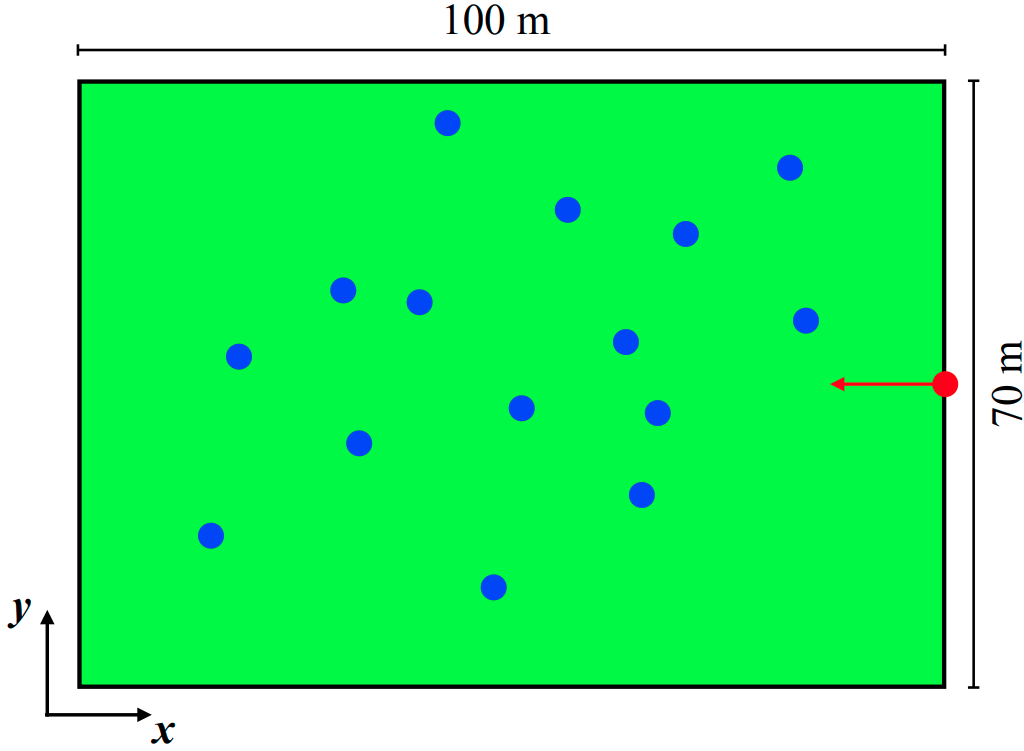
\includegraphics[width=0.7\textwidth]{pic/04-simulaciones/esquema-field}
        \end{minipage}
        \hfill
        \begin{minipage}{0.4\textwidth}
            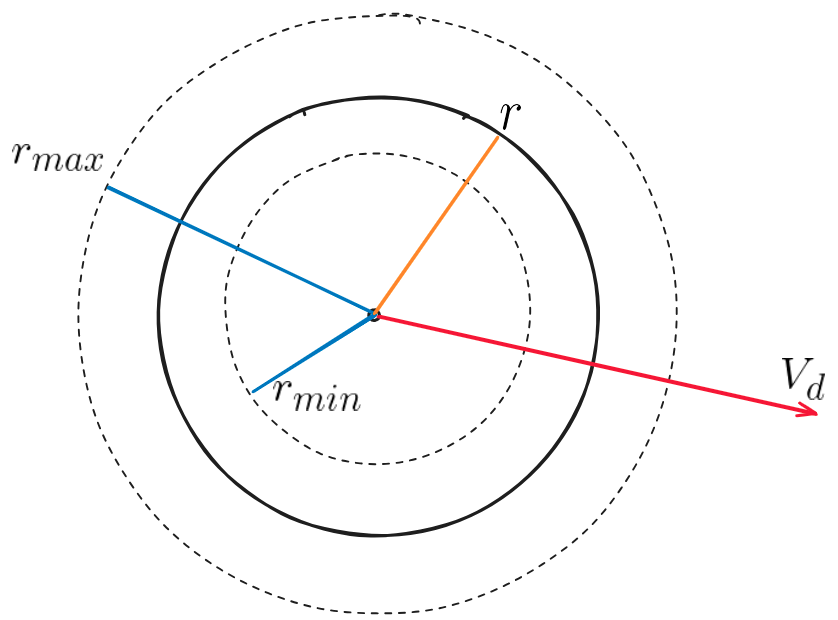
\includegraphics[width=\textwidth]{pic/04-simulaciones/esquema-particula}
        \end{minipage}
    \end{center}

    \footnotesize{
        \textbf{Consideraciones:}
        \begin{itemize}
            \item Se realizan 100 repeticiones por cada configuración.
            \item La posición inicial de los jugadores azules es uniformemente distribuida.
            \item La posición inicial del jugador rojo es fija, en el otro extremo de la cancha.
        \end{itemize}
    }

\end{frame}


\begin{frame}{Observables}
    \begin{block}{Distancia maxima recorrida en el eje x}
        Distancia máxima recorrida en la dirección x, promediada para todas las realizaciones.
        \begin{equation*}
            <|x - 100|>
        \end{equation*}
    \end{block}
    \begin{block}{Fracción de try logrados}
        Relación entre la cantidad de try's logrados $N_t$ y la cantidad de realizaciones $N_r$
        \begin{equation*}
            \Phi t = \frac{N_t}{N_r}
        \end{equation*}
    \end{block}
\end{frame}